\section{Affichage}

Dans ce projet, l'affichage est indispensable pour nous permettre d'avoir un appui visuel, certes les tests nous permettent de vérifier notre code, mais l'affichage visuel nous permet de mieux nous rendre compte de ce que nous faisons. Pour cela, nous avons deux manières d'afficher notre plateau, une manière primitive dans le terminal et une avec une interface web.

\subsection{Affichage primitif}

Dans un premier temps le but est d'afficher de manière simple, pour cela partant de l'implémentation vu en partie \ref{subsec:tile}. Pour cela nous utilisons des flèches "←↑" pour indiquer les entrées de route (ici "←↑" correspond à un type \texttt{Road} : \{$north$: true, $west$: true, $south$: false, $east$: false\}, 0 si il n'y a pas de route. Et pour les quartiers nous colorons le fond des flèches dans la couleur du quartier ce qui nous donne la tuile suivant en figure \ref{fig:tile_terminal}.


Ce premier affichage nous a permis de mieux avancer dans le projet mais il nous a fallu ensuite pouvoir voir le plateau décrit en partie \ref{subsec:board}. Comme celui-ci est représenté en \texttt{Quarter} il est facile de le représenter dans le terminale en trouvant l'ordonnée maximum et l'abscisse minimum puis d'afficher deux espaces si il n'y a pas de \texttt{Quarter} sinon afficher le \texttt{Quarter} et faire un retour a la ligne a chaque changement de ligne ce qui nous donne la figure \ref{fig:board_terminal}.

\begin{figure}[h]
    \centering
    \begin{minipage}{0.45\textwidth}
        \centering
        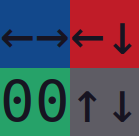
\includegraphics[width=0.5\linewidth]{images/Affichage/tile_termianl.png}
        \caption{Exemple d'affichage de tuile}
        \label{fig:tile_terminal}
    \end{minipage}\hfill
    \begin{minipage}{0.45\textwidth}
        \centering
        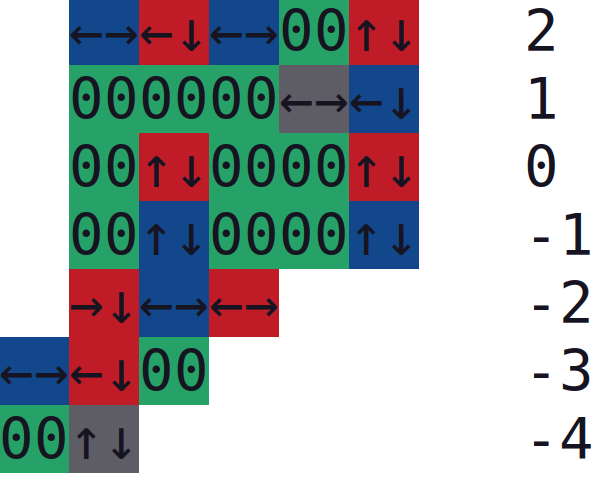
\includegraphics[width=0.5\linewidth]{images/Affichage/board_terminal.png}
        \caption{Exemple d'affichage du plateau}
        \label{fig:board_terminal}
    \end{minipage}
\end{figure}

\subsection{Affichage web}

Le projet proposait de créer une interface web permettant de visualiser des parties de Megalopolis. Cette interface, esthétiquement plus plaisante et interactive se fait à l'aide d'une page HTML, d'une feuille CSS et d'un script écrit en TypeScript permettant de lier notre page HTML au code réalisé pour le reste du projet.

\subsubsection{Interface graphique — HTML}

L'interface graphique se sépare en deux grands morceaux~: le plateau de jeu et le panneau de contrôle (voir Figure~\ref{fig:web_gui}).

\begin{figure}[h]
    \centering
    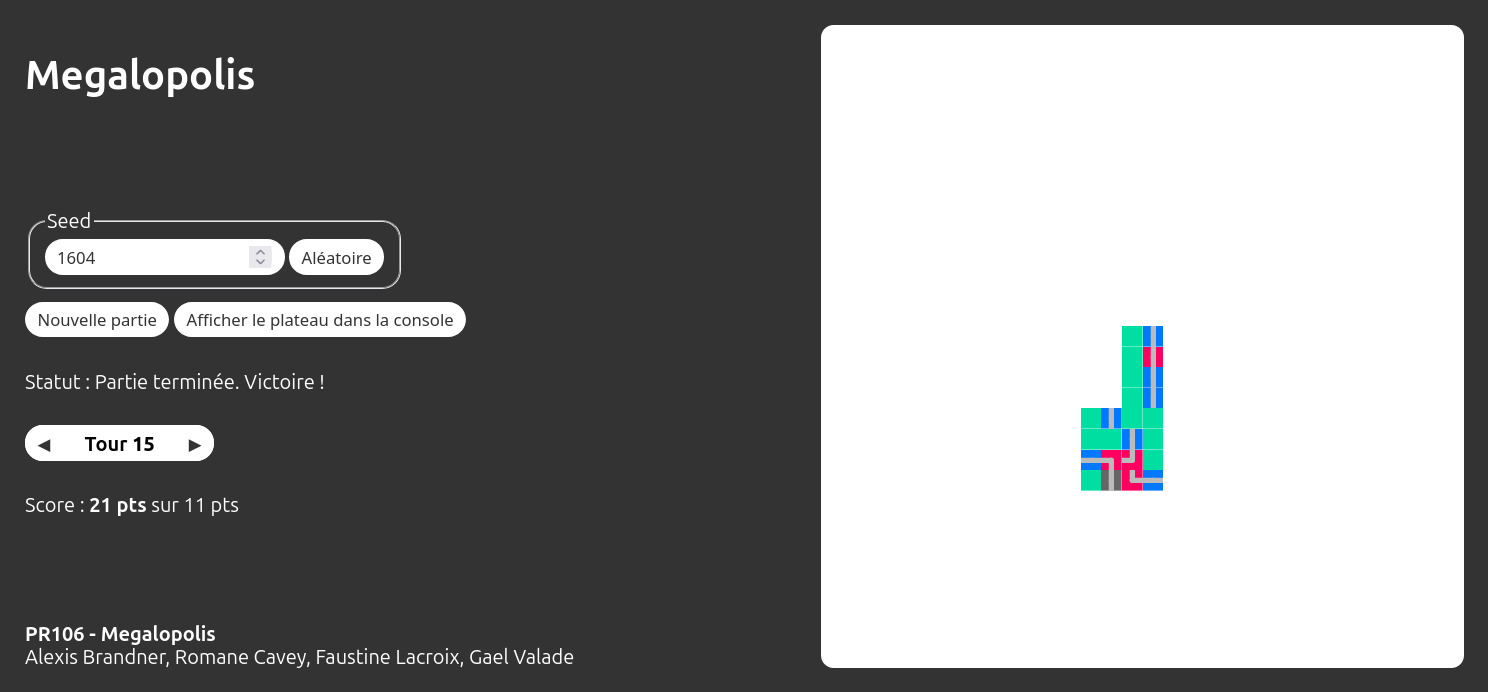
\includegraphics[width=0.75\linewidth]{images/Affichage/web-gui-v2.png}
    \caption{L'interface graphique}
    \label{fig:web_gui}
\end{figure}

Le plateau de jeu est représenté un élément \texttt{div}. Les tuiles sont découpées en quarts (comme dans le reste du jeu), qui sont placés dans le plateau. Le positionnement des quarts de tuiles sur le plateau se fait à l'aide d'une grille CSS et des propriétés \texttt{grid-column: x; grid-row: -y;} (l'axe des $y$ étant orienté vers le bas dans les grilles CSS).

Sur le plateau, chaque quart de tuile est représenté par un élément \texttt{svg} (dessin vectoriel). Ces dessins sont générés par le code, dessinant un rectangle pour la couleur de fond et deux lignes pour la route.

Le panneau de contrôle contient différents éléments~:
\begin{itemize}
    \item Un bouton permettant de lancer une partie
    \item Un bouton permettant d'avancer au tour suivant
    \item Un bouton permettant de retourner au tour précédent
    \item Un bouton permettant d'afficher la représentation textuelle du plateau dans la console du navigateur (utilisé pour le débugage)
    \item Un affichage de certaines informations utiles (n° du tour, score actuel, score requis pour gagner, etc.)
    \item Un champ permettant de spécifier une seed à utiliser
\end{itemize}

\subsubsection{Lien avec le reste du code — Interactivité}

Pour lier le reste du projet à notre interface graphique, on inclus dans le fichier \texttt{html/app.ts} (script associé à la page HTML, voir section~\ref{sec:parcel}) différents éléments provenant de nos autres fichiers de code. Afin de rendre l'exécution interactive, le code présent dans le fichier \texttt{src/main.ts} a été découpé 4 fonctions et copié dans un fichier \texttt{src/interactive.ts}. Le découpage suivant permet une exécution tour-par-tour de la partie, rendant l'affichage des premiers tours plus rapide~:

\begin{itemize}
    \item \texttt{initGame} : initialise une partie à partir d'une seed,
    \item \texttt{objScore} : calcule le score à atteindre pour remporter la partie,
    \item \texttt{playTurn} : joue une tour,
    \item \texttt{score} : calcule le score actuel.
\end{itemize}

Ces différentes fonctions sont appelées depuis \texttt{html/app.ts}, lorsque l'utilisateur appui sur certains boutons de la page (détection de l'évènement \texttt{click} avec la fonction \texttt{element.addEventListener}).

\subsubsection{Utilisation du bundler Parcel}

Parcel est un bundler permettant de livrer facilement une interface web. Parcel s'occupe de lancer localement un serveur web sur lequel va être hébergé une application. Cette application doit être fournie sous la forme suivante~:

\begin{itemize}
    \item Un document \texttt{index.html}, contenant la structure de la page web.
    \item Un script \texttt{app.ts}, qui est le script associé à la page. C'est ce script qui permettra de faire le lien entre le DOM (Document Object Model, qui contient les éléments HTML de notre page) et le code TypeScript que l'on a écrit pour l'application.
    \item Une feuille de styles \texttt{styles.css}, qui pourra contenir les différentes règles de mise en forme des éléments présents à l'écran.
\end{itemize}

% nécessite index.html, app.ts, et styles.css : compile les fichiers nécessaires & les distribue au client
% héberge localement

\label{sec:parcel}